% Made up for the tikra benchmark.
\usetikzlibrary{fit, positioning}
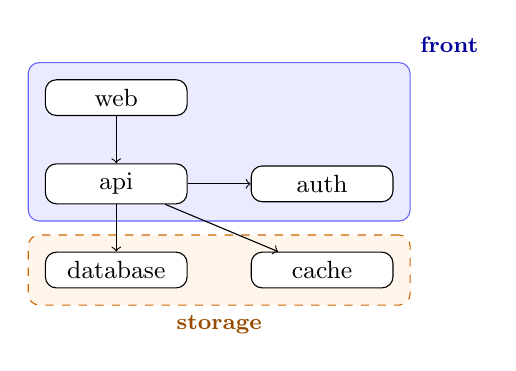
\begin{tikzpicture}[svc/.style={draw, rounded corners, fill=white, minimum width=1.8cm, font=\small}, node distance=6mm and 8mm]
  \node[svc] (web) {web};
  \node[svc, below=of web] (api) {api};
  \node[svc, right=of api] (auth) {auth};
  \node[svc, below=of api] (db) {database};
  \node[svc, right=of db] (cache) {cache};
  \node[draw=blue!60, fill=blue!8, rounded corners, inner sep=6pt, fit=(web) (api) (auth),
        label={[blue!60!black, font=\footnotesize\bfseries]north east:front}] (front) {};
  \node[draw=orange!80!black, dashed, fill=orange!8, rounded corners, inner sep=6pt, fit=(db) (cache),
        label={[orange!60!black, font=\footnotesize\bfseries]south:storage}] (store) {};
  \node[svc] at (web) {web};
  \node[svc] at (api) {api};
  \node[svc] at (auth) {auth};
  \node[svc] at (db) {database};
  \node[svc] at (cache) {cache};
  \draw[->] (web) -- (api);
  \draw[->] (api) -- (auth);
  \draw[->] (api) -- (db);
  \draw[->] (api) -- (cache);
\end{tikzpicture}
